% Review Thomas Schaller June 2020

%\usepackage{amssymb}
%\usepackage{mathtools}
%\usepackage{program}
%\setcounter{tocdepth}{3}
%\usepackage{graphicx}
%
%\usepackage{url}
%%\urldef{\mailsa}\path|{alexander.lawall, thomas.schaller, dominik.reichelt}@iisys.de|
%\urldef{\mailsa}\path|{firstname.lastname}@iisys.de|
%\usepackage[pdfpagelabels,hypertexnames=false,breaklinks=true,bookmarksopen=true,bookmarksopenlevel=2]{hyperref}





\chapter{Implementation of Subject-Oriented Models}



Subject oriented models address the internal aspects and structures of a system. They are essentially models of the internal structure of a system and cover organizational and technical aspects. When implementing the models, it is now necessary to establish the relationship between the process model and the available resources. Figure \ref{fig:Implementation-steps} shows the individual steps from a process model to the executable process instance.

\begin{figure}[h]
	\centering
	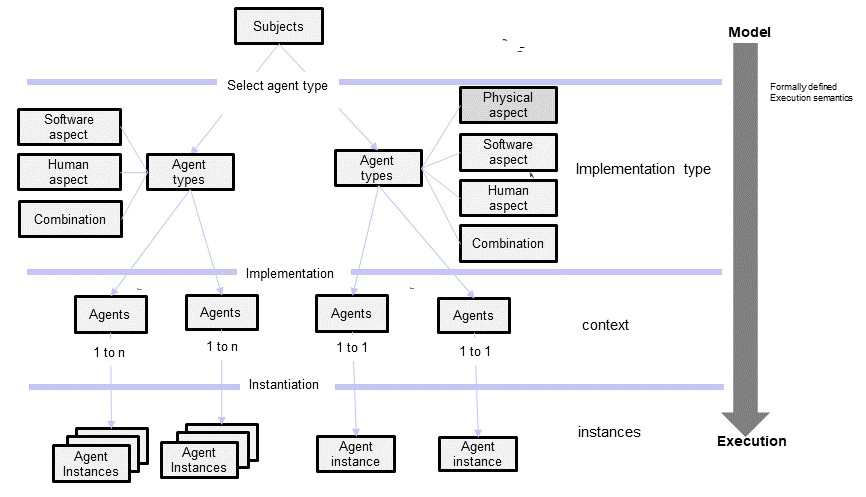
\includegraphics[width=0.9\linewidth]{Figures/Implementation/Implementation-steps.jpg}
	\caption[Implementation steps]{Implementation steps}
	\label{fig:Implementation-steps}
\end{figure}

In a system model, the actors, the actions, their sequences and the objects manipulated by the actions are described. Actions (activities) can be performed by humans, software systems, physical systems or a combination of these basic types of actors. We call them the task holders. For example, a software system can automatically perform the "tax rate calculation" action, while a person uses a software program to perform the "order entry" activity. The person enters the order data via a screen mask. The software checks the entered data for plausibility and saves it. However, activities can also be carried out purely manually, for example when a warehouse worker receives a picking order on paper, executes it, marks it as executed on the order form and returns it to the warehouse manager.\\
When creating a system model, it is often not yet known which types of actors execute which actions. Therefore, it can be useful to abstract from said CS: said?? the?  model when starting to describe processes by introducing abstract actors. A modeling language should allow the use of such abstractions. This means that when defining the process logic, no assertion should have to be made about what type of actor is realized. In S-BPM, the subjects represent abstract actors. \\
In the description of the control logic of a process, the individual activities are also described independently of their implementation. For example, for the action "create a picking order" it is not specified whether a human actor fills in a paper form or a screen mask, or whether a software system generates this form automatically. Thus, with activities the means by which something happens is not described, but rather only what happens.\\
The means are of course related to the implementation type of the actor. As soon as it has been defined which types of actors are assigned to the individual actions, the manner of realization of an activity has also been defined. In addition, the logical or physical object on which an action is executed also needs to be determined. Logical objects are data structures whose data is manipulated by activities. Paper forms represent a mixture between logical and physical objects, while a workpiece on which the "deburring" action takes place is a purely physical object. Therefore, there is a close relationship between the type of task holder, the actions and the associated objects actors manipulate or use when performing actions.\\
A system model can be used in different areas. The process logic is applied unchanged in the respective areas. However, it may be necessary to implement the individual actors and actions differently. Thus, in one environment certain actions could be performed by humans and in another the same actions could be performed by software systems. In the following, we refer to such different environments of use for a system model as context. Hence, for a process model, varying contexts can exist, in which there are different realization types for actors and actions.\\
In Subject Oriented Modeling, actors are not assigned to individual activities, but rather the actor type is assigned to an entire subject. This assignment is not part of the process logic, but in the most simple way it is done instead for each process in a separate two-column table. The left column contains the subject name and the right column the implementation type. If there are several contexts for a model, a separate assignment table is created for each of them.
The assignment of the implementation type forms the transition between the system logic and its implementation. Subsequently, it has to be defined which persons, software systems and physical systems represent the actors and how the individual actions are concretely realized. These aspects are described in detail in the following subsections.

\section{People and organizations}

This section describes how the organizational view of a company can be modeled formally and elements of it can be referenced with a modeling language.  Expressions of this language are stored in the subjects (the abstract actors) and resolved at runtime to a set of concrete actors. The actvities can then be assigned to them. 
The research presented here is able to represent any kind of resources of a company (people, software, machines etc.) and their arbitrary relationships amongst them. This way, the organizational structure of a company can be mapped very precisely.

The original idea of the approach goes back to Schaller's work  \cite{Schaller98}. Enhancements were made in the following articles \cite{Lawall2014, Lawall2014a, Lawall2014b, Lawall2014d, Lawall2014c, Lawall2013, Lawall2011}.

Let's start with the essential question whats makes up an organization. 


\subsection{What is an organization?}

\paragraph{Insights}
We are looking at a real world scenario in the context of an insurance company. 
A claims department usually has a manager, a number of clerks and a lawyer. Generally the lawyer is the deputy of the department head, cf. figure \ref{GeneralDep}.
	\begin{figure}[htb!]
	\centering
	\includegraphics[width=0.7\textwidth]{Figures/ExampleDepartmentGeneral.pdf}
	%\includegraphics[scale=0.65]{ExampleDepartmentGeneral.eps}
	\caption{Claims department in general}
	\label{GeneralDep}
	\end{figure}

We examined two concrete departments: one responsible for ``Car Damages'' the other responsible for ``House Damages''. Compared to the general structure and policies we observed some differences (cf. figure \ref{Example1}). At ``Car Damages'' there was an additional secretary position. In absence of the manager, organizational tasks were assigned to the secretary position. There was a change in the deputyship between the department head and the lawyer as well. Byron\footnote{We are using fantasy names.}, the lawyer, had been working in the department for only three weeks and therefore was not very experienced. The clerk Winter has been working in the department for over ten years. Based on that constellation the department head Smith decided that Winter should be his general deputy. Hinton was as well a deputy for Smith but only depending on some constraint information like the cash value of a claim for instance (constrained deputy relation in figure \ref{Example1}).

Looking at this two departments we also found an interesting mutual deputyship between the lawyers of the two departments (cf. figure \ref{Example1}). This observation gets important when thinking about dividing the organization system into types or classes on the one hand and instances on the other. Please note, that the relationships defined until now are specified on different levels of abstraction (positions and actors).
	\begin{figure}[htb!]
	\centering
	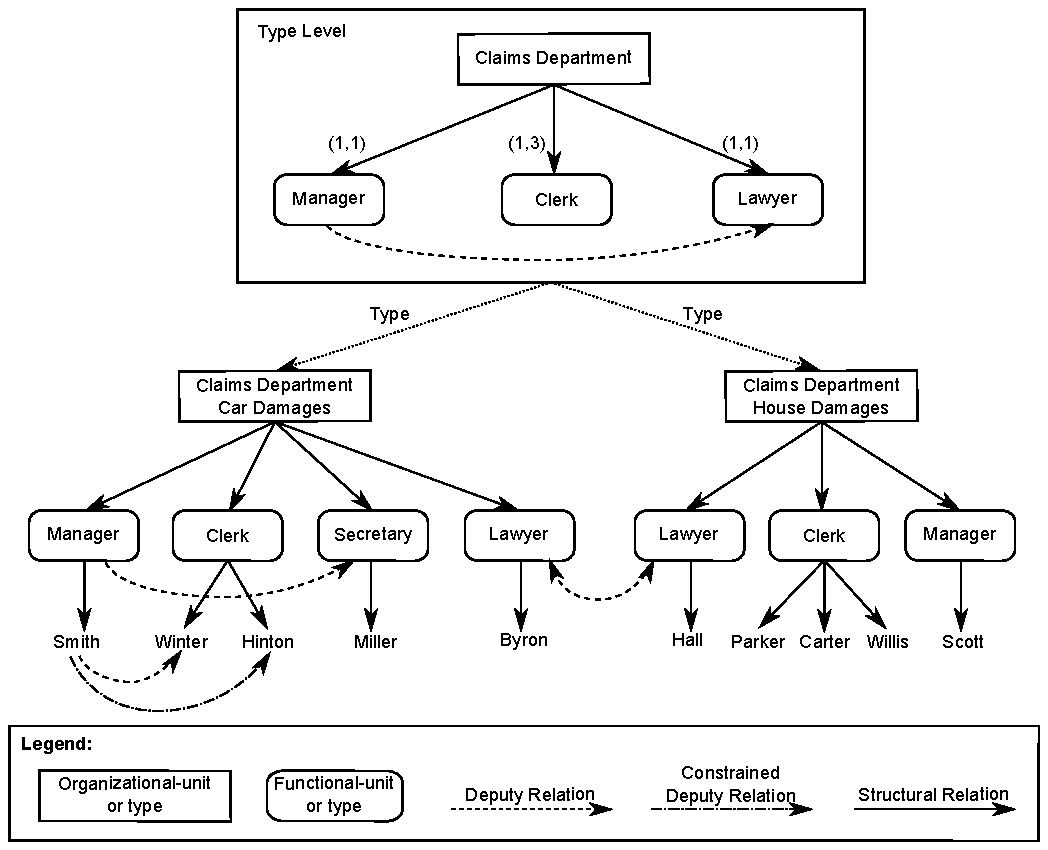
\includegraphics[width=\textwidth]{Figures/alles.pdf}
	\caption{Type and instance level of the example, adapted from \cite[fig. 3]{Lawall2013}}
	\label{Example1}
	\end{figure}

\subparagraph{Lessons Learned}

This section describes additional observations concerning real world organization policies\footnote{A complete overview can be found in \cite{Schaller98}.}.

\subparagraph{Knowledge Hierarchy}
As we have seen there are different levels of organizational knowledge. On the top level general structural assertions like ``a department consists of one to three clerks'' are dominant. We call this level the \emph{type} or \emph{template} level. Knowledge on this level is based on experience and is changed seldom as time goes by. Looking at real world departments -- we will call them \emph{instances} -- things become more concrete and specialized. There are concrete positions and the relationships between them. Finally, actors are assigned to the concrete positions. The organizational structures on this level are changing more frequently according to the demands of the daily business.

\subparagraph{Relationships}
An organization structure is formed by elements and relationships between them. It is important to realize the existence of several relationship types like ``is\_part\_of'', ``is\_deputy'', ``is\_supervisor'', ``reports\_to'' and so on.

Positions are abstractions of persons (actors) having a defined skill set fulfilling specific tasks. These abstractions help defining a more stable model of the organization that is independent from employee turnover. Relationships can be defined between abstract positions or on the concrete actor level.

Relationships are rarely of a general nature. As discussed in our example, relationships depend on specific constraint information like the cash value of a car claim. Even the ``is\_deputy''-relationship can depend on projects or products if you think in the terms of a matrix organization. They can also be only valid for a fixed time period.

\subparagraph{Multidimensional organizations}
Business organizations are multidimensional. Even in organizations that -- at first glance -- are structured hierarchically, there are structures belonging to the so called secondary (``shadow'') organization comprising committees, commissions, boards and so on. The positions and functions of the secondary organization are assigned to the employees. This leads to a multidimensional organization in every case. %We emphasize this point because there are some theories and approaches that are specific to hierarchical structures.

\subsection{Linking the process and the organizational model} \label{chapter_Linking}

Based on the organizational model, a server component is proposed that implements a special architecture and a unique algorithm for the resolution of expressions denoting abstract actors in the sense of subjects. This server is part of a greater system, the IT landscape of the company. ERP, process automation or database management systems can be other components of the landscape. Each of these systems uses mechanisms to map actors to tasks of processes or to permissions on data objects. Instead of maintaining such assignments for each system individually by total enumeration, we propose using an organizational server. This organizational server contains the organizational model. A formal language is used to formulate expressions that define the assignments. Clients send these expressions as requests to the organizational server and retrieve sets of real actors as reply (cf. figure \ref{architecture}). The server offers a versatile interface consisting of only one function \emph{dispatch} that returns a subset of the actors maintained within the organization model.

A major benefit of this approach is that the server forms the result set based on the current organizational model. This means that if actors change functions or relations, these changes have an immediate impact on the client systems. The language expressions remain unaltered. Before the organizational change, ``Manager(*)'' yields (according to fig. \ref{Example1}) the actors Smith and Scott. If Scott leaves the company and is replaced by Willis, the model is changed. Now, the same expression evaluates to Smith and the new manager Willis.

	\begin{figure}[htb!]
	\centering
	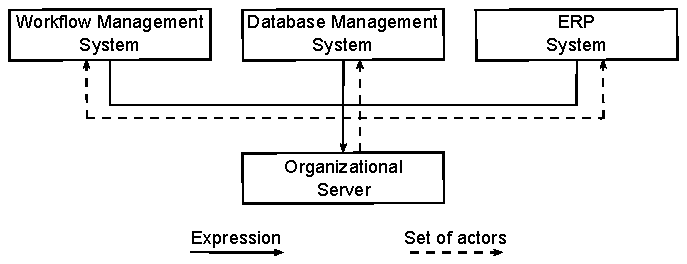
\includegraphics[scale=0.9]{Figures/architecture.pdf}
	\caption{Architecture}
	\label{architecture}
	\end{figure}

An informal overview on the functionality of the proposed server based on the introduced scenario could be assumed as the following. In a process management system a subject is defined by the expression  ``Manager(Claims Department Car Damages)''. At runtime the expression is passed to the organizational server. By traversing the organizational graph in figure \ref{Example1}, the algorithm moves to the department ``Claims Department Car Damages'' looking for a position ``Manager''. After that, the algorithm determines all the actors assigned to that position, finding manager Smith. If Smith is on the job, his identification is handed back to the workflow management system and the search ends. In case that Smith is not available (e.g. through vacation or sickness) the algorithm searches for  deputy relations between Smith and other actors. Obviously, there are two relations. If Winter \textbf{and} Hinton appear in the search result depends on the constraint on the relation to Hinton and whether they are on the job. In case of an empty set, the algorithm moves to the functional-unit manager looking 	for a deputy relation and finds the functional-unit secretary assigned to Miller. If Miller is on the job, her identification will be returned to the workflow management system. If not, the algorithm has the alternative of determining a valid deputy on the type level. Let us assume that the department is linked to the department type as depicted in figure \ref{Example1}. Within this type, the algorithm finds the lawyer as a deputy. It moves back to the instance ``Claims Department Car Damages'' and checks if there is a functional-unit with this name and an actor assigned to that functional-unit that is available. If Byron is on the job, his identification is returned. Otherwise, the lawyer of the ``Claims Department Car Damages'' has a two-way deputy relation with the lawyer of the ``Claims Department House Damages''. If this functional-unit has an actor assigned to itself and the actor is available, the algorithm will hand back his identification (here Hall, the lawyer of the ``Claims Department House Damages''). Otherwise the returned set is empty. In this case, the workflow management system has to postpone the execution of the task.


\section{Formal Specification}

The formalization of the organizational model is described using relations and integrity constraints. In the following we present a simplified model of Schaller's approach.

Within our meta-model an organization is a tuple O = ($name$, $\domaene$, $\OrgElementMenge$, $\relmenge$, $\relationen$) where $name$ denotes the modeled organization. The remaining symbols have the following semantics:

\subsection{Domains $\domaene$}
	$\domaene = \{ \Bezeichner, \zeit, \ID, \relname, \attribute, \WerteMenge, \praedikat \} $ is a set
	of domains consisting of the subsets:

	\begin{itemize}

	\item $\Bezeichner$ an organization specific set of terms describing the building blocks of the
	organization, like "`claims department"', department "`head"' and so on,

	\item $\zeit$ denotes a set of time values, like ``May 19th 2010 08:00:00''.

	\item $\ID$ a set of abstract identifiers.

	\item $\relname$ denotes a set of relationship names, "`deputy"' or "`reports\_to"' for instance.

	\item $\attribute$ a set of attributes used to detail the elements of our model. Attributes are mapped to model elements using the function  $val: \attribute \rightarrow \WerteMenge$ that assigns a value $w \in \WerteMenge$ to each
	$a \in \attribute$.

	\item	$\praedikat$ denotes a set of predicates like "`(ActualYear - HiringYear) $>$ 10"'.

	\end{itemize}

\subsection{Organization Elements $\OrgElementMenge$}
	The set $\OrgElementMenge = \oetyp \cup \ftyp \cup \oe \cup \f \cup \a $ comprises all the building blocks of an organization on the type as well as on the instance level. The elements of $\OrgElementMenge$ represent the nodes of the resulting organization graph.

	\begin{itemize}

	\item $\oetyp$ denotes the set of organizational-unit types, like departments or working groups.


	\item $\ftyp$ is the set of functional-unit types, like the ``manager'', ``lawyers''\ and so on.


	\item $\oe$ represents the set of organizational-units, like departments, committees, teams and so on. As already explained, organizational-units can have a relation to a type. The total function $type_{\oe}: \oe \rightarrow \oetyp \cup NULL$ returns the specific type for every organizational-unit.

	\item $\f$ is the set of functional-units, like positions or roles. There also exists a type function that is almost defined in the same manner as described above. The type of a functional-unit is returned by the function $type_F{\f}: \f \rightarrow \ftyp \cup NULL$.

	$\relstrukturOE_F \subset \oe \times (\oe \cup \f)$ denotes the is\_part\_of-relation between organizational- and functional-units.$\relstrukturOE_F$ on the one hand	describes the mapping of functional-units to organizational-units. On the	other hand the hierarchy between orga-nizational-units can be modeled. When focusing on the organizational-units the relation ${\relstrukturOE_F}^{'} = \relstrukturOE_F \rhd \oe$ has to be irreflexive and cycle-free. ${\relstrukturOE_F}^{''} = \relstrukturOE_F \rhd \f$ has to be surjective.

	\item  $R^{\f}$ denotes a set of user-defined relations. All members $r \in R^{\f}$ have the structure $r \subset (\f \times \f)$ and	are irreflexive.

	\item The set $\a$ denotes the actors: employees (users) and the computer systems. We explicitly model these computer systems because they can carry out tasks and therefore need permissions. $\relstrukturFA \subset \f \times \a$ is a relation and describes the assignments of employees to positions. As seen before, there is also a user-defined set of relationships $R^{\a}$. All relations $r \in R^{\a}$ have the structure $r \subset (\a \times (\a \cup \f))$. Further on, for all $r \in R^{\a}$ the condition $\forall r \in R^{\a}: \left[(x,y) \in r \rightarrow x \neq y \right]$ holds, meaning that every relation	$r \in R^{\a}$ is cycle-free.

	\item Additionally every element of $\OrgElementMenge$ is described as tuple $(id, name)$, with $id \in \ID$ and $name \in \Bezeichner$.

	\end{itemize}

\subsection{Set of Relations $\relmenge$}
	$\relmenge$ denotes a set of relation sets and is defined as
	$\relmenge = \relmengetyp \cup \relmengeinst$, with:

	\begin{itemize}

	\item $\relmengetyp$ denotes the set of relations defined between the types of organizational- and functional-units.
	$\relmengetyp$ is defined as $\relmengetyp = \typstrukturrelation \cup \typbenutzerrelationenmenge$, with:
	\begin{itemize}

		\item $\typstrukturrelation \subset \oetyp \times (\oetyp \cup \ftyp)$ is the ``is\_part\_of''-relation on the type level. Concerning the structure between the elements of $\oetyp$, there are some restrictions. Let's say ${\typstrukturrelation}^{'} = \typstrukturrelation \rhd \oetyp$\footnote{The operator $\rhd$ is defined as $((\rel \subset A \times B) \rhd (C \subset B)) := \{(x,y) \in \rel \, \vert \, y \in C \}$.}.
		An organizational-unit type can not be his own successor. ${\typstrukturrelation}^{'}$ therefore has to be irreflexive and cycle-free.
		Let's have a look at the functional-unit types. Obviously the relationship between $\oetyp$ and $\ftyp$ can be described as ${\typstrukturrelation}^{''} = \typstrukturrelation \rhd \ftyp$. Since organizational-unit types combine functional-unit types, ${\typstrukturrelation}^{''}$ has to be total. On the other side, every $f \in \ftyp$ has to be linked to an organizational-unit type $o \in \oetyp$. ${\typstrukturrelation}^{''}$ therefore has to be surjective.

		\item As explained above, there is the need for a flexible integration of new relation-types into the model. Therefore we define a set of relation-types $\typbenutzerrelationenmenge$. Every relationship $\typbenutzerrelation \in R^{\typsymbol}$ has the structure $\typbenutzerrelation \subset (\ftyp \times \ftyp) \times \praedikat$ and can further be constraint using predicates to restrict the set of valid functional-unit types and therefore the set of valid users\footnote{Please take a look at the relation $\relstrukturFA$ and its according constraints}. Please note that $\typbenutzerrelation$ is used as variable. The relations between the functional-unit types, that can expressed using the term $dom(\typbenutzerrelation)$, are irreflexive. Defining a deputyship between one node and itself is not very meaningful for instance. Concerning the predicates we additionally postulate that each $\typbenutzerrelation \in \typbenutzerrelationenmenge$ has to be a function, assigning each ordered pair $(f,f) \in \ftyp \times \ftyp$ a unique predicate $p \in \praedikat$.

	\end{itemize}
	\item $\relmengeinst$ defines several relations between organizational- and functional-unit types as well as actors. We declare $\relmengeinst$ as 		$\relmengeinst = \relmengeinstOE_F \cup \relmengeinstFA$, with:

		\begin{itemize}

		\item $\relmengeinstOE_F = \relstrukturOE_F \cup \relmengebenutzerinstOE_F$ the set of relations between organizational- and functional-units, with:
			\begin{itemize}
			\item $\relstrukturOE_F \subset \oe \times (\oe \cup \f)$ denotes the ``is\_part\_of''-relation between organiza-tional- and functional-units. On the one hand the relation describes the functional-units belonging to an organizational-unit, on the other hand the organization structure between the units themselves. Let ${\relstrukturOE_F}^{'} = \relstrukturOE_F \rhd \oe$ denote the structure between the organizational-units. According to our description ${\relstrukturOE_F}^{'}$ has to be irreflexive and cycle-free. In the same manner and similar to our definition of ${\typstrukturrelation}^{''}$,${\relstrukturOE_F}^{''} = \relstrukturOE_F \rhd \f$ has to be total and surjective.

			\item $\relmengebenutzerinstOE_F$ is a set of user-defined relations. Every single relation ${\relbenutzerinstOE_F}$ within $\relmengebenutzerinstOE_F$ has the structure ${\relbenutzerinstOE_F} \subset \f \times \f$ and is irreflexive.
			\end{itemize}

		\item $\relmengeinstFA$ denotes a set of relations between functional-units and actors. $\relmengeinstFA$ is defined as $\relmengeinstFA = \relstrukturFA \cup \relmengebenutzerFA$, with:

			\begin{itemize}

			\item $\relstrukturFA \subset \f \times \a$ describes the function assignments of the actors. We demand that every actor is named to at least one function.

			\item $\relmengebenutzerFA$ a set of user-defined, irreflexive relations 	${\relbenutzerFA}$ having the structure $\forall {\relbenutzerFA} \in \relmengebenutzerFA: {\relbenutzerFA} \subset \a \times (\a \cup \f)$. For every $\relbenutzerFA \in \relmengebenutzerFA$ the condition		$\left[(x,y) \in \relbenutzerFA \rightarrow x \neq y \right]$ holds.
			\end{itemize}

		\end{itemize}

	\end{itemize}

	All elements of our model can be detailed using time constraints and attributes.

\subsection{Additional relations $\relationen$}

	$\relationen$ consists of several relations and is defined as $\relationen =\{ \rel_{Time}, \rel_{\attribute},$ $\rel_{Card}, \rel_{val}, \rel_{Name}\}$, with:

	\begin{itemize}
	\item $\rel_{Time} \subset \bigl( \OrgElementMenge \cup \relmenge \bigr)\times \bigl( \zeit \times \zeit \bigr)$ describes the duration of validity of every single organizational element in our model. $\rel_{Time}$ therefore has to be a total relation.

The two functions $start$ and $stop$ denote the birth and death of an organizational element. We define these functions as:
			$$
			\begin{array}{cll}
			start: \bigl( \OrgElementMenge \cup \relmenge \bigr) \rightarrow \zeit, &
				\mbox{with the semantic} & \\
				& start(x \in ( \OrgElementMenge \cup \relmenge ) ) =
				dom( ran ( x \lhd \rel_{Time})) & \\
			stop: \bigl( \OrgElementMenge \cup \relmenge \bigr) \rightarrow \zeit, &
				\mbox{with the semantic} & \\
				& stop(x \in ( \OrgElementMenge \cup \relmenge ) ) =
				ran( ran ( x \lhd \rel_{Time})) & \\
			\end{array}
			$$
It is obvious that the following constraint should hold: $\forall x \in \bigl( \OrgElementMenge \cup \relmenge \bigr): start(x) \leq stop(x)$.  In order to define an existence ad infinitum we introduce the symbol ``$*$''\ concerning the value of the $stop$ function.

	\item $\rel_{\attribute} \subset \bigl( \OrgElementMenge \cup \relmenge \bigr) \times \attribute$ assigns attributes to our organizational elements.
		$\rel_{\attribute}$ is a surjective relation. Thus every attribute can only be assigned to one organizational element.

	\item $\rel_{Card} \subset \typstrukturrelation \times (\natnull \times \natnull)$ assigns cardinalities to our ``is\_part\_of''-relation between organizational- and functional-unit types. $\rel_{Card}$ is a total and unique relation.

		As abbreviations we define the functions $min$ and $max$, with
		$$
		\begin{array}{cl}
		min: \typstrukturrelation \rightarrow \natnull, & \mbox{with the semantic} \\
		& min(r \in \typstrukturrelation) = dom( ran( r \lhd \rel_{Card})) \\
		max: \typstrukturrelation \rightarrow \natnull, & \mbox{with the semantic} \\
		& max(r \in \typstrukturrelation) = ran( ran ( r \lhd \rel_{Card}))
		\end{array}
		$$
		Additionally we demand $\forall r \in \typstrukturrelation: min(r) \leq max(r)$.

	\item Via $\rel_{val} \subset \praedikat \times (\f^{\typsymbol} \cup A)$ each predicate, its typed functional-unit and actors is assigned. The predicate {\em true} holds for all typed functions and actors and we define $\forall x \in \f^{\typsymbol} \cup A: \quad (true, x) \in \rel_{val}$.

	\item $\rel_{Name} \subset \bigl( \typbenutzerrelationenmenge \cup \relmengebenutzerinstOE_F \cup \relmengebenutzerFA \bigr) \times \relname$
		assigns names to our user-defined relations. None of these relations should be nameless. $\rel_{Name}$ therefore has to be total and unique.
		As already mentioned, $\typstrukturrelation, \relstrukturOE_F$ and	$\relstrukturFA$ denote ``is\_part\_of''-relations. A specific naming of these 		relations is therefore unnecessary.
\end{itemize}

\subsection{Policy Resolution}\label{PolicyResolutionFormal}

As discussed in section \ref{chapter_Linking} our organizational server offers an interface with a very small footprint, consisting only of the function "`dispatch"'. The function returns a subset of the actors fulfilling the language expression in conjunction with conditions. These conditions are formulated via the following parameters expected by the function.
\begin{itemize}
	\item a set of organizational-unit names $oe_{bez} \in \Bezeichner$,
	\item a set of tuples consisting of attributes and corresponding values $attr_{oe} \subset (\Bezeichner \times \WerteMenge)$ belonging to defined organizational-units,
	\item a set of functional-unit names $f_{bez} \in \Bezeichner$,
	\item a set of tuples consisting of attributes and corresponding values $attr_{f} \subset (\Bezeichner \times \WerteMenge)$ belonging to functional-units,
	\item a set of actor names $a_{bez} \in \Bezeichner$,
	\item a set of tuples consisting of attributes and related values $attr_{a} \subset (\Bezeichner \times \WerteMenge)$, belonging to actors,
	\item the name of a relation $rel \in \relname$ and
	\item a set of tuples consisting of attributes and corresponding values $attr_{rel} \subset (\Bezeichner \times \WerteMenge)$, belonging to that relation.
\end{itemize}

%The {\tt dispatch}-algorithm works as follows:

	\begin{samepage}
	{\small
	\NumberProgramstrue
	\begin{algorithm}[dispatch]\label{alg:GetIt}
	\begin{program}
	\FUNCT |dispatch|(oe_{bez} \subset \Bezeichner, attr_{oe} \subset (\Bezeichner \times \WerteMenge),
	f_{bez} \subset \Bezeichner, attr_f \subset (\Bezeichner \times \WerteMenge),
	a_{bez} \subset \Bezeichner, attr_a \subset (\Bezeichner \times \WerteMenge),
	rel \in \relname, attr_{rel} \subset (\Bezeichner \times \WerteMenge)) \subset \a
	\BEGIN
	\var \seq{oe \subset \oe; f \subset \f; a \subset A};
	/*|First we have to determine the existing organizational elements|*/
	oe := (\oe \rhd oe_{bez});
	f := (\f \rhd f_{bez});
	a := (A \rhd a_{bez});
	\IF (oe \neq \{\} \vee attr_{oe} \neq \{\}) \label{alg:GetIt:CallGetATbyOE}
	\THEN \RETURN \quad GetATbyOE(oe, attr_{oe}, f, attr_f, rel, attr_{rel})
	\FI
	\IF (f \neq \{\} \vee attr_f \neq \{\})
	\THEN \RETURN \quad GetATbyF(f, attr_f, attr_a, rel, attr_{rel})
	\FI
	\IF (a \neq \{\} \vee attr_a \neq \{\})
	\THEN \RETURN \quad GetAT(a, attr_a, rel, attr_{rel})
	\FI
	\RETURN \{\};
	\END
	\end{program}
	\end{algorithm}
	\NumberProgramsfalse
	}
	\end{samepage}

\noindent The execution of {\tt dispatch(\{Claims Department Car Damages\},\{\},\{Clerk\},\\ \{\},\{\},\{damage sum $<$ \$100\},\{\},\{\})} is equivalent to search all clerks in the organizational-unit {\it car damages} that are authorized to sign claims with a damage sum lower than 100 dollars. The execution will lead to a call of the {\tt GetATbyOE}-function. Based on the values of $oe$, $f$ and $a$ {\tt GetATbyOE} determines the organization elements fulfilling the remaining conditions specified in $attr_{oe}$, $attr_{f}$ and so on.

	%\longpage
	\begin{samepage}
	{\small
	\NumberProgramstrue
	\begin{algorithm}[GetATbyOE]\label{alg:GetATbyOE}
	\begin{program}
	\FUNCT |GetATbyOE|(oe \subset \oe, attr_{oe} \subset (\Bezeichner \times \WerteMenge), f \subset \f,
	attr_{f} \subset (\Bezeichner \times \WerteMenge), rel \in \relname, attr_{rel} \subset (\Bezeichner \times \WerteMenge),
	attr_a \subset (\Bezeichner \times \WerteMenge)) \subset \a
	\BEGIN
	\var \seq{f^{'} \subset \f; oe_{successor},oe_{successor}^{'} \subset \oe;
		o_{p} \subset \oe \times \oe};
	%=====================================================================================
	%\IF attr_{oe} = \{\} \THEN attr_{oe} = \attribute \FI \label{alg:GetATbyOE:kritisch1}
	%=====================================================================================
	/* o_{p}| denotes the vector corresponding to oe|*/;
	o_{p} := \{(x,y) \vert x \in oe \wedge y \in \oe \};\label{alg:GetATbyOE:Vektor}
	oe_{successor} := dom \left( \left({\left({\left({\relstrukturOE_F}^{'}\right)}^{*}\right)}^{T}\right) \circ o_{p} \right);\label{alg:GetATbyOE:Nachfolger}
	\IF (oe_{successor} = \{\})
	\THEN oe_{successor} := \oe; \label{alg:GetATbyOE:kritisch2}
	\FI
	%=======================================================================================
	%oe_{Nachfolger}^{'} := dom( \{ oe_{Nachfolger} \} \lhd \rel_{\attribute} \rhd attr_{oe} )
	%=======================================================================================
	oe_{successor}^{'} := GetOrgElements( oe_{successor}, attr_{oe});
	\IF (f = \{\})\label{alg:GetATbyOE:fIstNull}
	\THEN
		/*|determine all functional-units of the organizational-units|*/
		f^{'} := ran ( \{oe_{successor}^{'}\} \lhd \relstrukturOE_F ) \cap F;
		\RETURN \quad |GetATbyF|(f^{'}, attr_{f}, attr_a, rel, attr_{rel});
	\ELSE \label{alg:GetATbyOE:fIstNichtNull}
		/*|which of the preselected functional-units belong to|*/
		/*|the organizational-units determined in |oe_{successor}^{'}?*/
		f^{'} := ran ( \{oe_{successor}^{'}\} \lhd \relstrukturOE_F \rhd \{f\}) \cap F;
		\RETURN \quad |GetATbyF|(f^{'}, attr_{f}, attr_a, rel, attr_{rel});
	\FI
	\RETURN \quad \{\};
	\END
	\end{program}
	\end{algorithm}
	\NumberProgramsfalse
	}
	\end{samepage}

\noindent Line \ref{alg:GetATbyOE:Vektor} describes the declaration of a relational vector. The calculation of all successors in line \ref{alg:GetATbyOE:Nachfolger} is obtained by multiplying the transpose of the irreflexive closure of ${\relstrukturOE_F}^{'}$ with our vector $o_{p}$. After that we select the appropriate organizational-units.\\

In the case of the functional-unit set $f$ passed to our function is empty, the algorithm selects all functional-units of the calculated transitive-reflexive closure and calls the function {\tt GetATbyF} (line \ref{alg:GetATbyOE:fIstNull}). If $f$ != $\{\}$ the relevant functional-units are selected in dependency on the specified organizational-units. After that the function {\tt GetATbyF} is called	(line \ref{alg:GetATbyOE:fIstNichtNull}).

	%\longpage
	\begin{samepage}
	{\small
	\NumberProgramstrue
	\begin{algorithm}[GetATbyF]\label{alg:GetATbyF}
	\begin{program}
	\FUNCT |GetATbyF|(f \subset \f, attr_f \subset (\Bezeichner \times \WerteMenge), attr_a \subset (\Bezeichner \times \WerteMenge),
	rel \in \relname, attr_{rel} \subset (\Bezeichner \times \WerteMenge)) \subset \a
	\BEGIN
	\var \seq{f^{'},f^{''} \subset \f; a \subset A};
	\IF (attr_f = \{\})
	\THEN attr_f := \attribute;
	\FI
	f^{'} := f;
	\IF (f^{'} = \{\})
	\THEN f^{'} := \f;
	\FI
	%==========================================================
	%f^{'} := dom ( \{f\} \lhd \rel_{\attribute} \rhd attr_f );
	%==========================================================
	f^{''} := GetOrgElements( f^{'}, attr_f );
	a := ran( f^{''} \lhd \relstrukturFA );
	\RETURN \quad |GetAT|(a, attr_a, rel, attr_{rel});
	\END
	\end{program}
	\end{algorithm}
	\NumberProgramsfalse
	}
	\end{samepage}

\noindent Function {\tt GetATbyF} determines the set of functional-units fulfilling the attributes passed over as parameters first. After that corresponding actors are selected and handed over to {\tt GetAT}.\\

Algorithm \ref{alg:GetAT} describes the core idea of our system. The passed parameters are being processed from the actor level up to level of organizational- and functional-unit types. Individual rules therefore have a higher priority than policies specified on the more abstract type level.

	{\small
	\NumberProgramstrue
	\begin{algorithm}[GetAT]\label{alg:GetAT}
	\begin{program}
	\FUNCT |GetAT|(a \subset \a, attr_a \subset (\Bezeichner \times \WerteMenge), rel \in \relname, attr_{rel} \subset (\Bezeichner \times \WerteMenge)) \subset \a
	\BEGIN
	\IF (attr_a = rel = attr_{rel} = \{\})\label{alg:GetAT:trivial}
	\THEN \RETURN \quad a;
	\FI
	/* |exit for recursions| */
	\IF (attr_a \neq \{\} \wedge (rel = attr_{rel} = \{\})) \label{alg:GetAT:Aussprung}
	\THEN
		\IF a = \{\} \THEN a := \a \FI \label{alg:GetAT:A-Erweiterung}
		%=======================================================================================
		%a := dom \bigl( \{a\} \lhd \rel_{\attribute} \rhd \{attr_a\} \bigr); \label{alg:GetAT:1}
		%=======================================================================================
		\RETURN \quad  GetOrgElements( a, attr_a ); \label{alg:GetAT:1}
	\FI
	\IF rel \neq \{\} \label{alg:GetAT:komplex}
	\THEN
		\IF a = \{\} \THEN a := \a \FI
		%=======================================================================================
		%\IF attr_{rel} = \{\} \THEN attr_{rel} := \attribute \FI
		%=======================================================================================
		\var \seq{\rel_x, \rel_x^{'} \in \relmengebenutzerFA; y \subset (\f \cup \a)};
		/* | is there a user-defined relation fulfilling the attributes?|*/
		%\rel_x^{'} := name^{-1}(rel) \cap \relmengebenutzerFA; \label{alg:GetAT:FA}
		\rel_x^{'} := dom(\rel_{Name} \rhd rel) \cap \relmengebenutzerFA; \label{alg:GetAT:FA}
		%=======================================================================================
		%\rel_x := dom(\{\rel_x^{'}\} \lhd \rel_{\attribute} \rhd attr_{rel});
		%=======================================================================================
		\rel_x := GetOrgElements( \rel_x^{'}, attr_{rel});
		\IF \rel_x \neq \{\}
		\THEN
		%=======================================================================================
		%	z := ran ( dom ( (\{a\} \lhd \rel_x) \lhd \rel_{\attribute} \rhd \{attr_{rel}\} ) );
		%=======================================================================================
			\var \seq{z \subset A \cup \f; w,y \subset A};
			z := ran( GetOrgElements(\{a\} \lhd \rel_x, attr_{rel}) );
			/*| select the actors according to |$z$
			w := z \cap \a;
			/*| select the actors according to | \relstrukturFA */
			y := ran (\{ \{z\} \cap \f\} \lhd \relstrukturFA);
			\RETURN \quad w \cup y;
		\ELSE
			\var \seq{\rel_x^\f, {\rel_x^\f}^{'} \subset \relmengebenutzerinstOE_F};
			%{\rel_x^\f}^{'} := name^{-1}(rel) \cap \relmengebenutzerinstOE_F; \label{alg:GetAT:FF}
			{\rel_x^\f}^{'} := dom(\rel_{Name} \rhd rel) \cap \relmengebenutzerinstOE_F; \label{alg:GetAT:FF}
			%===================================================================================
			%\rel_x^\f := dom(\{{\rel_x^\f}^{'}\} \lhd \rel_{\attribute} \rhd attr_{rel});
			%===================================================================================
			\rel_x^\f := GetOrgElements({\rel_x^\f}^{'}, attr_{rel});
			\IF \rel_x^\f \neq \{\}
			\THEN
				\var \seq{a^{'} \subset A};
				/*|select all actors connected to the functional-unit |*/
				a^{'} := ran \left( \{ ran \left( \rel_x^\f \right) \} \lhd \relstrukturFA \right);
				\RETURN \quad |GetAT|(a^{'}, attr_a, \{\},\{\});
			\ELSE /*|lookup in the  type level|*/
			\var \seq{\rel_x^\ftyp,{\rel_x^\ftyp}^{'} \subset \typbenutzerrelationenmenge};
			%{\rel_x^\ftyp}^{'} := name^{-1}(rel) \cap \typbenutzerrelationenmenge; \label{alg:GetAT:FtFt}
			{\rel_x^\ftyp}^{'} := dom(\rel_{Name} \rhd rel) \cap \typbenutzerrelationenmenge; \label{alg:GetAT:FtFt}
			%===================================================================================
			%\rel_x^\ftyp := dom(\{{\rel_x^\ftyp}^{'}\} \lhd \rel_{\attribute} \rhd attr_{rel});
			%===================================================================================
			\rel_x^\ftyp := GetOrgElements({\rel_x^\ftyp}^{'}, attr_{rel});
			\IF \rel_x^\ftyp \neq \{\}
			\THEN
				\var \seq{f^{'},f^{''} \subset \f; a^{'},a^{''},a^{'''} \subset A};
				/*|1. address all true relationships |*/ \label{alg:GetAT:PraedikateStart} \label{alg:GetAT:WahrePraedikate}
				%/*|mit dem Pr"adikat "`wahr"'|*/
				f^{'} := dom \bigl( type_F^{\typsymbol} \rhd ran( dom (\rel_x^\ftyp \rhd \{wahr\}))\bigr);
				a^{'} := ran \bigl( f^{'} \lhd \relstrukturFA \bigr);
				/*|2. address false relationships |*/\label{alg:GetAT:NichtWahrePraedikate}
				%/*|Pr"adikaten ungleich "`wahr"'|*/
%				/* */
				/*|2.1 address typed functional-units |*/
				f^{''} := dom \bigl( \bigl( type_F^{\typsymbol} \rhd ran( dom (\rel_x^\ftyp \rrhd wahr\})) \bigr)
				\cap
				ran \bigl( ran(\rel_x^\ftyp \rrhd \{wahr\}) \lhd \rel_{val} \bigr) \bigr);
				a^{''} := f^{''} \lhd \relstrukturFA;
				/*|2.2 address direct relationships|*/
			a^{'''} :=
				\bigl( dom \bigl( type_F^{\typsymbol} \rhd ran( dom (\rel_x^\ftyp \rrhd \{wahr\})) \lhd \relstrukturFA \bigr)
				  \cap ran \bigl(  ran(\rel_x^\ftyp \rrhd \{wahr\}) \lhd \rel_{val} \bigr) \bigr);
				\RETURN \quad |GetAT|(a^{'} \cup a^{''} \cup a^{'''}, attr_a, \{\},\{\}); \label{alg:GetAT:PraedikateStop}
			\ELSE
				/*| no corresponding relationship found |*/

				\RETURN \quad \{\};
			\FI
		\FI
	\FI
	\FI
	\END
	\end{program}
	\end{algorithm}
	\NumberProgramsfalse
	}

\noindent Line \ref{alg:GetAT:trivial} describes the trivial case. If the only parameter is a set of actors the return value will be the same set.\\

In case that attributes are handed over (that have to be fulfilled by the respective actors) and no user-defined relation was defined (line~\ref{alg:GetAT:Aussprung}), the algorithm determines all actors with a fulfilling attribute set. If $a$ is empty, all actors (line \ref{alg:GetAT:A-Erweiterung}) are used within the search (line \ref{alg:GetAT:1}). \\

The core concept of the algorithm starts with line \ref{alg:GetAT:komplex}. The following user-defined relations have to be resolved:
\begin{itemize}
	\item The relation between actors and functional-units ($\relmengebenutzerFA$),
	\item The relation between functional-units ($\relmengebenutzerinstOE_F$) and
	\item The relation between functional-unit types ($\typbenutzerrelationenmenge$)
\end{itemize}

If no corresponding relation on the actor level can be found (line \ref{alg:GetAT:komplex}), the algorithm checks for a connection between two functional-units ($\relmengebenutzerinstOE_F$) in order to retrieve the attached actors. If no match is possible, the algorithm searches for a relation on the more abstract type level (line \ref{alg:GetAT:FtFt}). If a relation can be found these policies are used for retrieving matching actors on the instance level. Lines \ref{alg:GetAT:PraedikateStart} to \ref{alg:GetAT:PraedikateStop} show the semantics of the predicates $p \in \praedikat$ of the relation $\typbenutzerrelation \in \typbenutzerrelationenmenge$. All not predicate constrained relations are evaluated (line \ref{alg:GetAT:WahrePraedikate}), first. After that the algorithm examines the constrained relations (line \ref{alg:GetAT:NichtWahrePraedikate}).  The resulting actor set is used for a recursive call of algorithm \ref{alg:GetAT}.\\

\noindent Algorithm {\tt GetOrgElements} selects those elements fulfilling a defined attribute set $attr$ from the set of organizational-units and relations.

	%\longpage
	\begin{samepage}
	{\small
	\NumberProgramstrue
	\begin{algorithm}[GetOrgElements]\label{alg:GetOrgElements}
	\begin{program}
	\FUNCT |GetOrgElements|(k \subset \OrgElementMenge \cup \relationen, attr \subset (\Bezeichner \times \WerteMenge)) \subset \OrgElementMenge \cup \relationen
	\BEGIN
	\var \seq{ x \subset \OrgElementMenge \cup \relationen};
	x := \{\};
	\FOREACH y \in k~\DO
		\IF CheckAttributes(y, attr)
		\THEN
			x := x \cup y;
		\FI
	\OD
	\RETURN \quad x;
	\END
	\end{program}
	\end{algorithm}
	\NumberProgramsfalse
	}
	\end{samepage}

\noindent The following algorithm checks if an attribute of set $attr$ is mapped to an organizational element or relation $k \in \OrgElementMenge \cup \relationen$.

	\begin{samepage}
	{\small
	\NumberProgramstrue
	\begin{algorithm}[CheckAttributes]\label{alg:CheckAttributes}
	\begin{program}
	\FUNCT |CheckAttributes|(k \in \OrgElementMenge \cup \relationen, attr \subset (\Bezeichner \times \WerteMenge)) \subset \boole
	\BEGIN
	\var \seq{attr_k \subset \attribute};
	\IF (attr = \{ \})
		\THEN \RETURN \quad \true;
	\ELSE
		attr_k := ran( k \lhd \rel_{\attribute});
		\IF ( dom(attr) \subset ran( attr_k ))
		\THEN
			\FOREACH y \in attr~\DO
				\IF (ran(y) \neq val(attr_k \rhd dom(y)))
				\THEN \RETURN \quad \false;
				\FI
			\OD
			\RETURN \quad \true;
		\ELSE \RETURN \quad \false;
		\FI
	\FI
	\END
	\end{program}
	\end{algorithm}
	\NumberProgramsfalse
	}
	\end{samepage}

\noindent If the required attributes and attribute values are mapped to an organizational element or relation, function {\tt CheckAttributes} returns $true \in \boole$, or otherwise $false \in \boole$. $\boole = \{ true, false \}$ denotes the set of boolean values.

\section{Implementation}
The formalism discussed in this contribution is implemented in a prototype. Figure \ref{proto-gui} depicts part of this implementation -- the graphical user interface (GUI). It contains a \emph{model} editor, a \emph{search} area, a \emph{tree-navigation} as well as an \emph{attribute pane} and a \emph{relation list} for a selected organizational element.

\begin{figure}
\centering
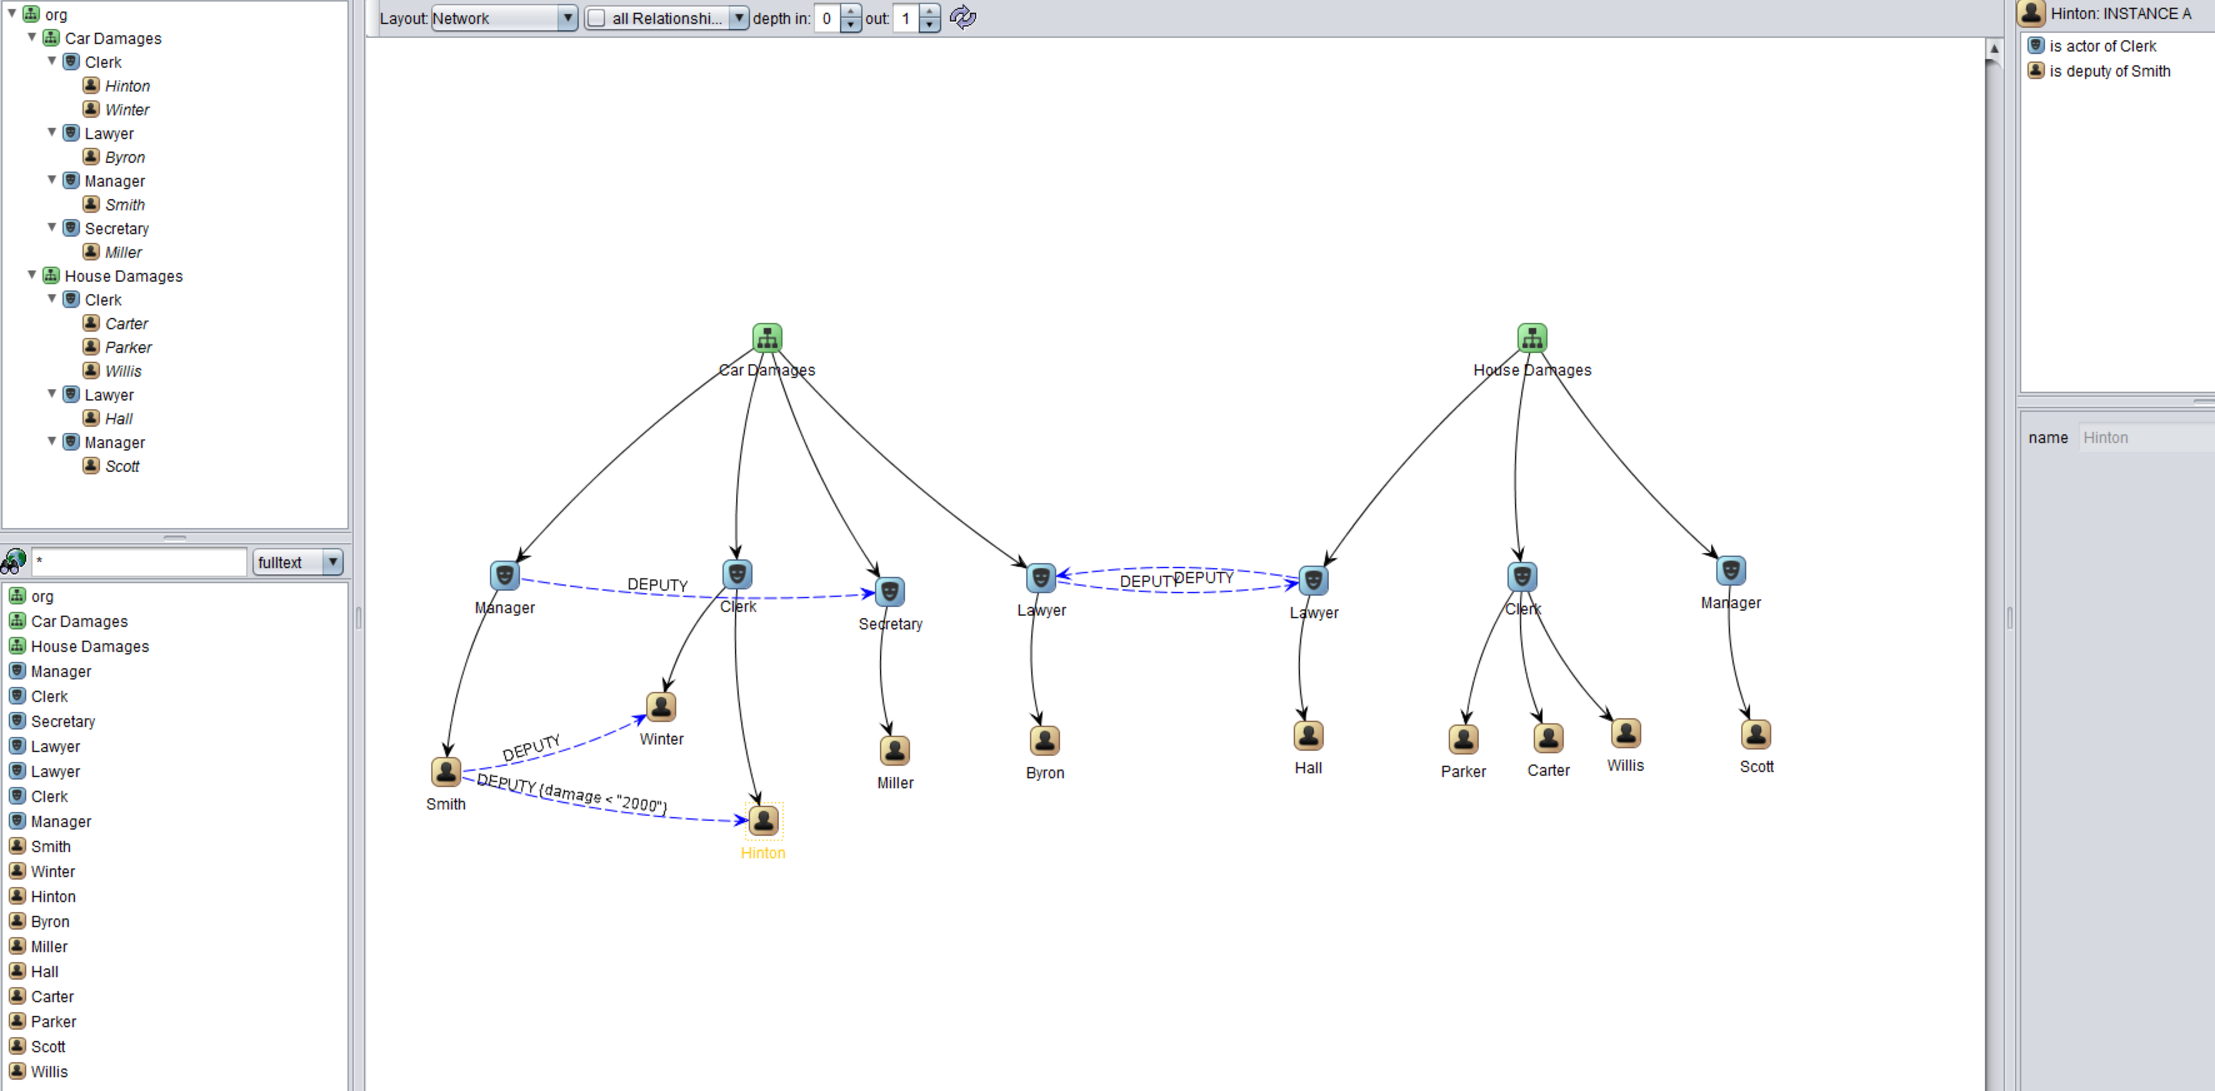
\includegraphics[width=\textwidth]{Figures/corg}
\caption{Screenshot: Implementation of the $\mathcal{C-ORG}$} GUI
\label{proto-gui}
\end{figure}

\begin{description}
  \item[The \emph{model editor}] provides a graph-based view on the organizational structure. Organizational elements are represented as nodes and their relations as edges. It provides means to navigate the model by centering on selected nodes. As the central component of the user interface, it is discussed below in more detail.
	\item[The \emph{search area}] can be used to retrieve a list of organizational elements. It has two modes of operation:
	  \begin{enumerate}
		  \item It provides a simple text index search for attribute values, e.g. entering ``Wi*'' will yield Winter and Willis.
			\item It can also be used to evaluate language expressions based on the approach described in section  and \ref{PolicyResolutionFormal}. An expression is entered and the result set for the current state of the organizational model is shown.
		\end{enumerate}
	\item[The \emph{tree-navigation}] projects the concrete organizational structure on a tree. Consequently, entities are duplicated in the projection if they can be reached on different paths.
	\item[The \emph{attribute pane}] in the bottom right section shows the attributes of the currently selected node or relation. It allows a quick modification, e.g. the assignment of a predicate to a relation.
	\item[The \emph{relation list}] lists all relations of the currently selected node, independent from the relation-types hidden in the model editor. This allows access to connected nodes and significantly reduces the time required to alter existing relations.
\end{description}

For quick access, elements can be dragged from any of the outer GUI sections and dropped into the model editor. If the elements have existing relations to the nodes already shown in the model editor, these relations will be shown as well. Otherwise, the elements are represented as unconnected nodes.

\begin{figure}
\centering
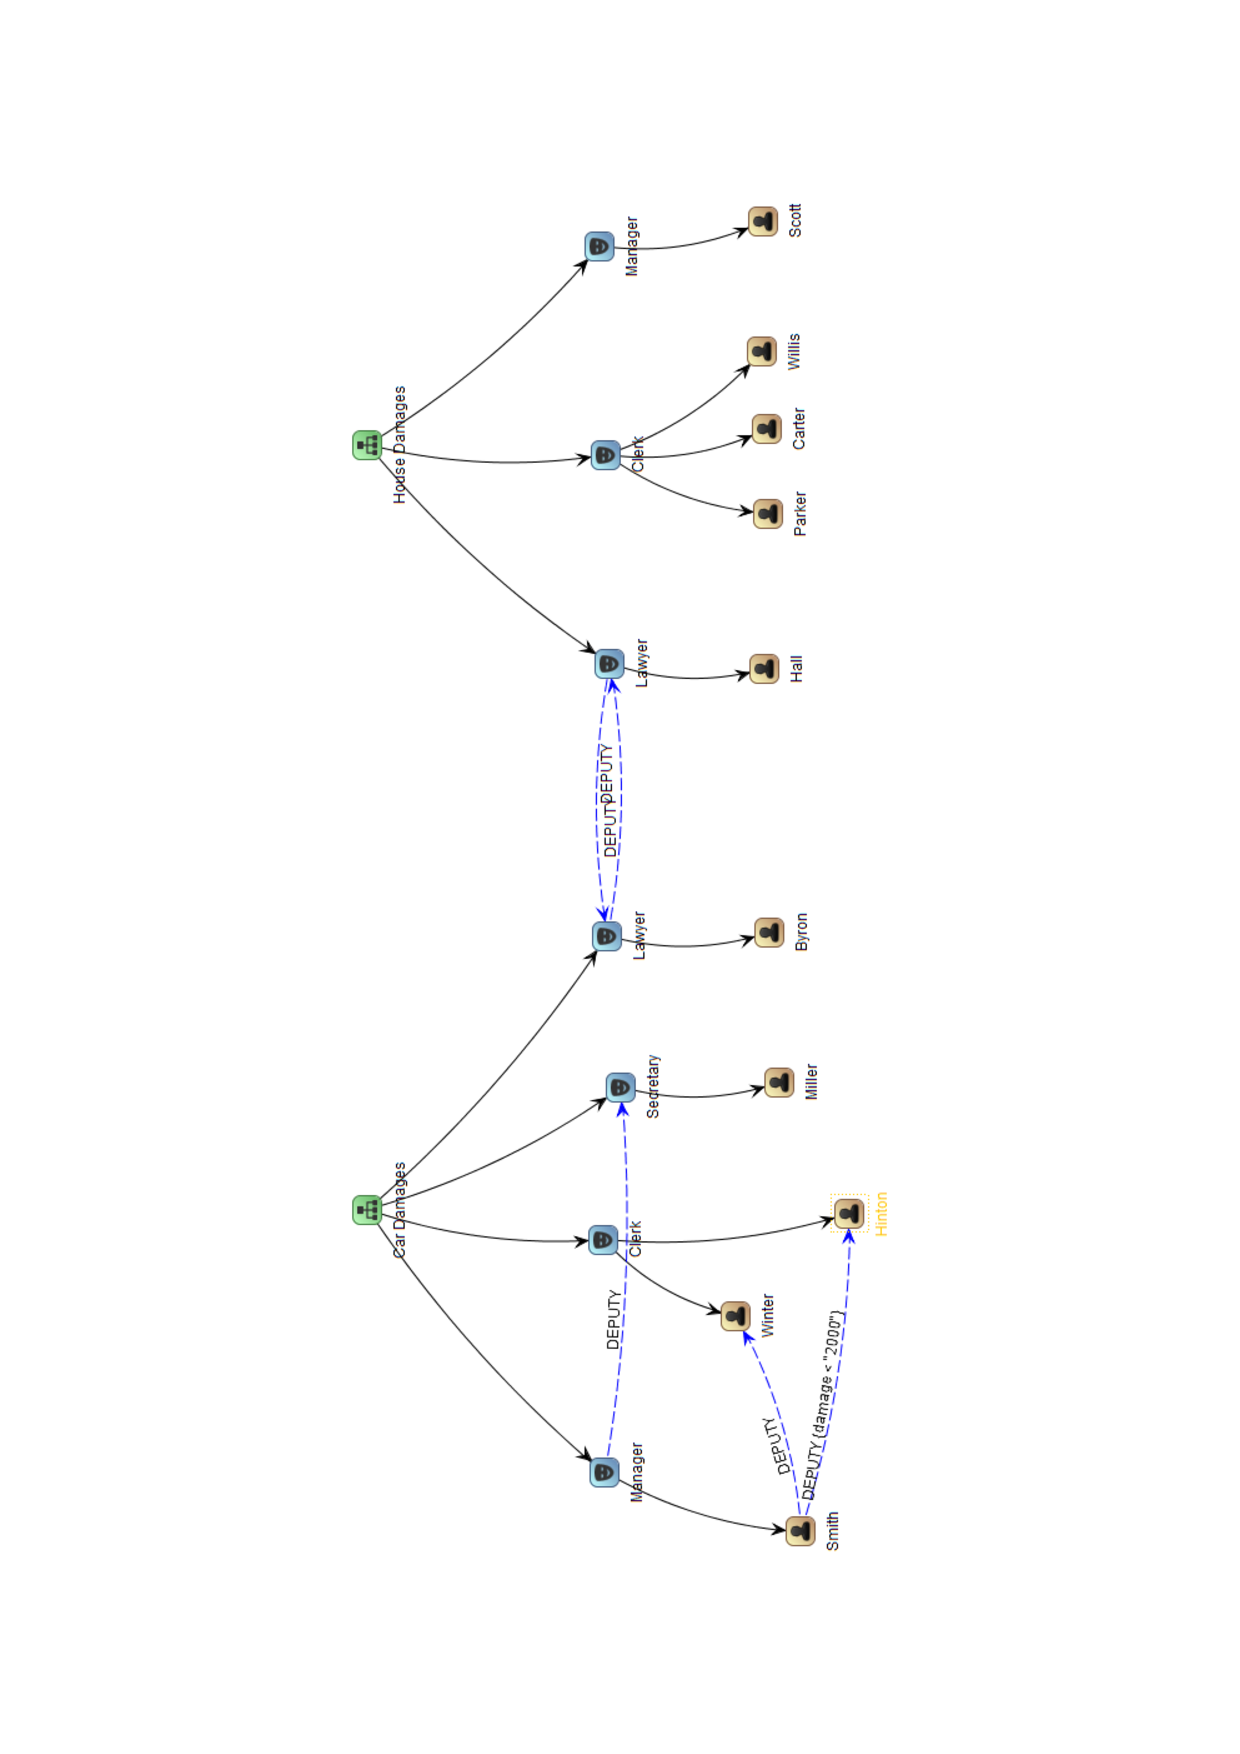
\includegraphics[width=\textwidth]{Figures/corg-graph.pdf}
\caption{Model Region of the Implementation}
\label{proto-model}
\end{figure}

Figure \ref{proto-model} provides an enlarged view of the model editor\footnote{It shows the example model (cf. fig. \ref{Example1}). The type level is hidden.}.
Users perform most modifications of the organizational model via this component.
In addition to navigating the model, they can create, modify and delete organizational elements and their interconnections.

It contains the model with the desired\footnote{The relation-types to be shown can be selected.} relations. The editor also shows concrete constraints (predicates) on relations, e.g. the deputy relation with \emph{damage $<$ ``2000''} between \emph{Smith} and \emph{Hinton}.


In addition to the user interface, the implementation provides a service that can accept language expressions from client systems. This interface is based on the Representational State Transfer (REST) paradigm.



\section{Physical infrastructure}

\todo{Bibtex-File muss noch angepasst werden.}

The previous remarks always referred to human actors. But executors in a business process can also be machines or software components. We will therefore look at how the concept presented in the previous chapters can be extended to the area of non-human actors. Here, the already introduced concepts such as substitutions are also used. 

Let us take a look at the Industry 4.0 area. 

Production plants as we know them today are actually overthought within the smart factories initiative. Central production plans for manufacturing big numbers of similar products are replaced by intelligent objects embedded in self-organizing systems called smart factories \cite{Gronau2015}. These objects are cyber-physical systems \cite{meissner2013} using intelligent sensors for gathering information about the world around them.  They are able to react to environmental changes and to generate plans for fulfilling their goals. So, if a customer orders a product at a manufacturing company an agent responsible for the production of the article is created. This agent knows all about the bill of material and the working plan for the creation of the product. On basis of this information the agent generates a plan how the product can be manufactured. For this he has to talk other agents representing the resources of the company. 

%In this article we show a graph-based approach for maintaining the resources of a smart factory and searching for them using a declarative query language. This language can be used by the production agent looking for resources that are able to fulfill manufacturing tasks of the working plan.

%\subsection{Organizational Model} \label{modell} 

\begin{figure*}[htb!]
	\centering
	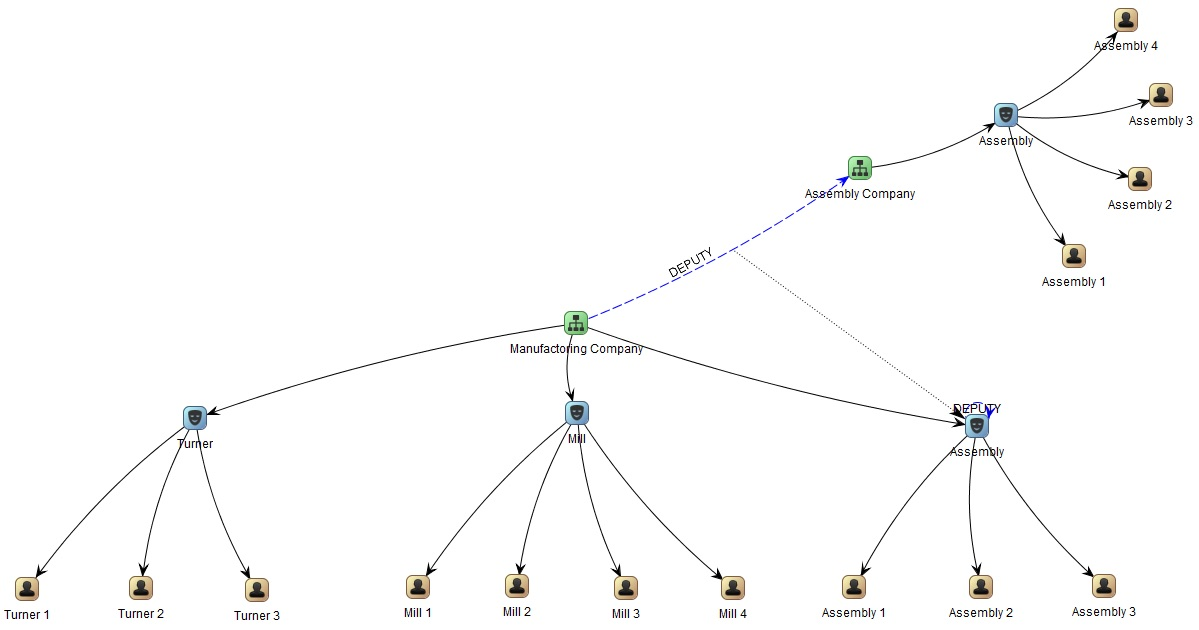
\includegraphics[width=\textwidth]{Figures/orgamodelfed.jpg}
	\caption{Federation between Partner Companies}
	\label{fig:federation}
\end{figure*}

Figure \ref{fig:federation} depicts an excerpt of the organizational model of a manufacturing company producing wooden chairs. The model encompasses the internal organizational unit \emph{Manufacturing Company} with the subordinate internal functional units \emph{Turner}, \emph{Mill} and \emph{Assembly}. The internal resources \emph{Turner 1} to \emph{Turner 3} are related to \emph{Turner}, \emph{Mill 1} to \emph{Mill 4} belong to \emph{Mill} and \emph{Assembly 1} to \emph{Assembly 4} are part of the internal functional unit \emph{Assembly}. 

The properties and capabilities of the elements of the organization can be described using attributes. In our example, the maximum length of a workpiece to be processed and the shape of a workpiece on the machines is of interest.
Table \ref{tab:intagents}  describes an excerpt of attributes in conjunction with their values. 

%The table \ref{tab:intagents} depicts attribute-value pairs of internal automatic resources of the \emph{Manufacturing Company}.
\begin{table}[htb!]
	\centering
	\begin{tabular}{|l||l|l|}
		\hline
		Resource & Attribute & Value \\ 
		\hline
		\hline
		Turner 1 & minworkpieceLength & 30 \\
		\hline 
		& maxworkpieceLength & 50\\
		\hline
		& workpieceKind & octagonal\\
		\hline
		&...&...\\
		\hline
		Turner 2 & minworkpieceLength & 35\\
		\hline
		& maxworkpieceLength & 40\\
		\hline
		& workpieceKind & octagonal\\
		\hline
		&...&...\\
		\hline
		Turner 3&minworkpieceLength & 40 \\
		\hline
		& maxworkpieceLength & 50\\
		\hline
		& workpieceKind & square\\
		\hline		
		&...&...\\
		\hline
		Mill 1& maxLength & 100cm \\
		\hline
		& maxWidth & 100cm\\
		\hline
		& maxHeight & 20 cm\\
		\hline
		Mill 2& .... & ... \\
		\hline
		Assembly1 & Type & 304456\\
		\hline
		& ... & ...\\
		\hline
		Assembly2(PC) & Type & 304456\\
		\hline
		& ... & ...\\
		\hline
	%	&...&...\\
	%	\hline
	%	Mill 3& & \\
	%	\hline
	%	&...&...\\
	%	\hline
	%	Mill 4& & \\
	%	\hline
	%	&...&...\\
	%	\hline
	%	Assembly 1& & \\
	%	\hline
	%	&...&...\\
	%	\hline
	%	Assembly 2& & \\
	%	\hline
	%	&...&...\\
	%	\hline
	%	Assembly 3& & \\
	%	\hline
	%	&...&...\\
	%	\hline
	\end{tabular} 
	\caption{Attributes of Resources} 
	\label{tab:intagents}
\end{table}

Looking at the relationships there exists an external partner company (assembly company) that can take over assembly tasks on load peaks
\footnote{The automated propagation of model elements (entities, relations and attributes) to partner organizations is described in \cite{Lawall2014a}.}. The federation between the manufacturing company and the assembly company extends the aforementioned organizational model. The external organizational unit \emph{Assembly Company} encompasses the external functional unit \emph{Assembly} in conjunction with the external resources \emph{Assembly 1} to \emph{Assembly 4}. 

%So a partner company can act as a proxy. This substitution is described in detail using attributes and hyperedges. For a deeper understanding, please refer to the article \cite{Lawall2014a}.  

Finding the correct agent for a specific task is done by resolving an organzational language expression that is defined in the subject specification.
The expression can reference entities, relations and/or attributes. 
Suppose a production agent wants to have 64 chair legs manufactured for the production of a batch of chairs of type 304456. He first looks in the master data record to see what specifications the legs must have. He finds a length of 40 cm and octagonal shape. He can use these two specifications to find a suitable machine. The expression looks like this:\\

\texttt{(Turner)(Manufacturing Company). ATT.(minworkpieceLength $\leq$ "40" AND maxworkpieceLength $\geq$ AND workpieceKind = "octagonal")}\\

This means the production agent is looking for an agent of type "`turner"' that is able to produce workpieces with length 40cm and an octogonal form.The
search is local to the manufacturing company. In our example, turning machines 1 and 2 are eligible for the production step.
Finding a production resource to manufacture the 64 seats and backrests works on the same principle. Now the chairs still have to be assembled. The agent finds a suitable assembly unit with the following query:\\

\texttt{ (Assembly)(*).ATT.\\(Model $=$ "304456"))} \\
 
The asterisk means that substitutions are also permitted for this request. Thus, the company's own production facility (Assembly 1) as well as the machine of the partner company (Assembly 2) can be found. Depending on the degree of workload of the resources, the agent decides whether he then locks the order on his own machine or the machine of the partner company. \\

Similar to production resources, software products, actuators or sensors can be modelled and managed according to the same principle. 


%\section{IT-Systems and Software}
